\section{Technical Papers}
\subsection{ZoeMatrope: A System for Physical Material Design}
\frame
{
	\frametitle{ZoeMatrope: A System for Physical Material Design}
	ZoeMatrope: A System for Physical Material Design \cite{Miyashita:2016}
	
	\begin{figure}
		\centering
		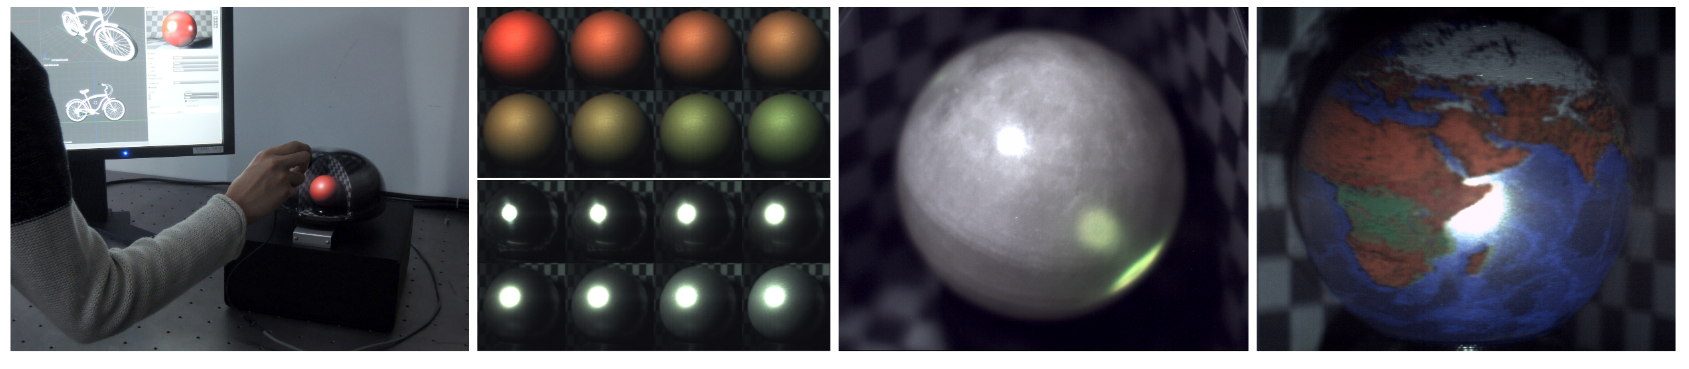
\includegraphics[width=1.0\textwidth]{img/zoematrope/zoematrope.png}
	\end{figure}
}

\frame
{
	\frametitle{ZoeMatrope: A System for Physical Material Design}
	
	\begin{figure}
		\centering
		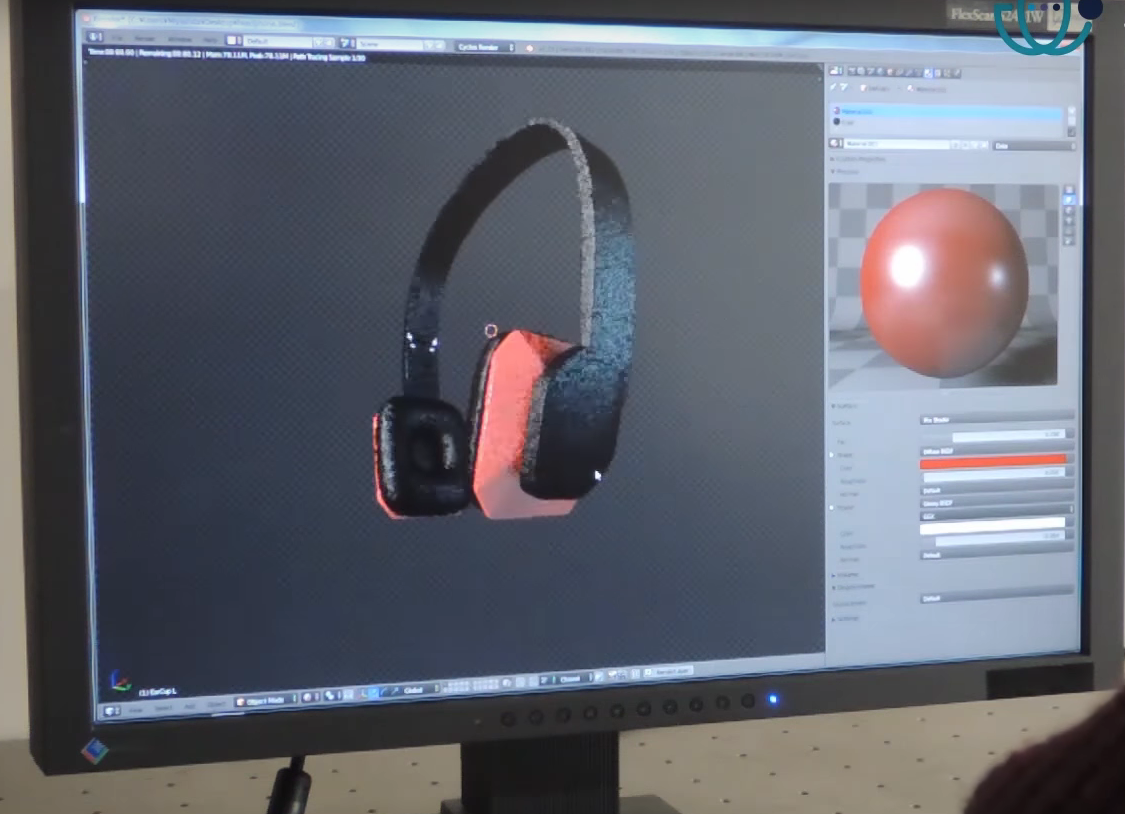
\includegraphics[width=0.5\textwidth]{img/zoematrope/design.png}
	\end{figure}
	
	\begin{itemize}[<+->]
		\item Context: 3D product design
		\item Challenges: Variety of materials, resolution, dynamic range
		\item \textit{Reality is the most realistic representation}
	\end{itemize}
}

\frame
{
	\frametitle{ZoeMatrope: A System for Physical Material Design}
	\centering
	Thaumatrope
	\begin{figure}
		\centering
		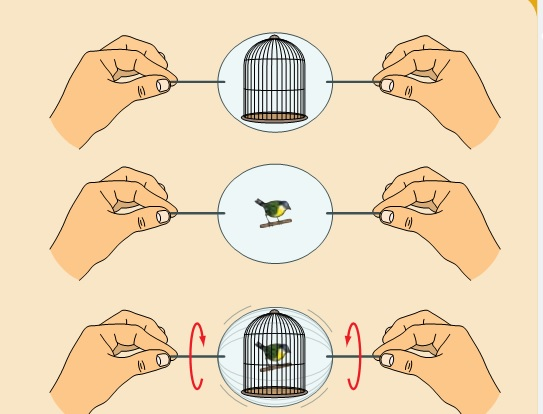
\includegraphics[width=0.7\textwidth]{img/zoematrope/thaumatrope.jpg}
	\end{figure}
	
}

\frame
{
	\frametitle{ZoeMatrope: A System for Physical Material Design}
	\begin{figure}
		\centering
		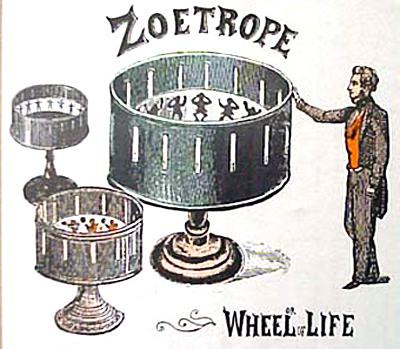
\includegraphics[width=0.6\textwidth]{img/zoematrope/zoetrope.jpg}
	\end{figure}
	
	\centering
	\url{https://www.youtube.com/watch?v=5khDGKGv088&t=23s}
}

\frame
{
	\frametitle{ZoeMatrope: A System for Physical Material Design}
	ZoeMatrope: A System for Physical Material Design \cite{Miyashita:2016}
	
	\centering
	\url{https://www.youtube.com/watch?v=w0ZPvTYzbsc&t=19s}
}

\subsection{Perspective-aware Manipulation of Portrait Photos}
\frame
{
	\frametitle{Perspective-aware Manipulation of Portrait Photos}
	Perspective-aware Manipulation of Portrait Photos \cite{Fried:2016}
	
	\begin{figure}
		\centering
		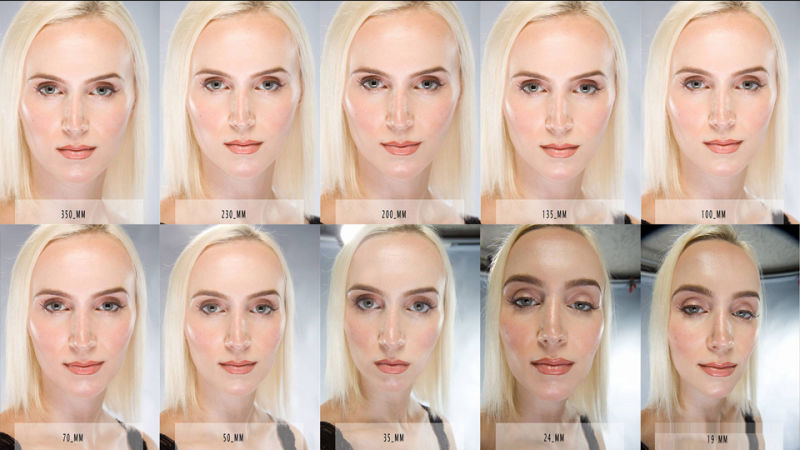
\includegraphics[width=0.9\textwidth]{img/perspective/portraitlens.jpg}
	\end{figure}
}

\frame
{
	\frametitle{Perspective-aware Manipulation of Portrait Photos}
	
	
	\begin{enumerate}
		\item Fiducial detection
		\item Parametrized 3D head model fitting
		\item Manipulation
	\end{enumerate}
	
	\begin{figure}
		\centering
		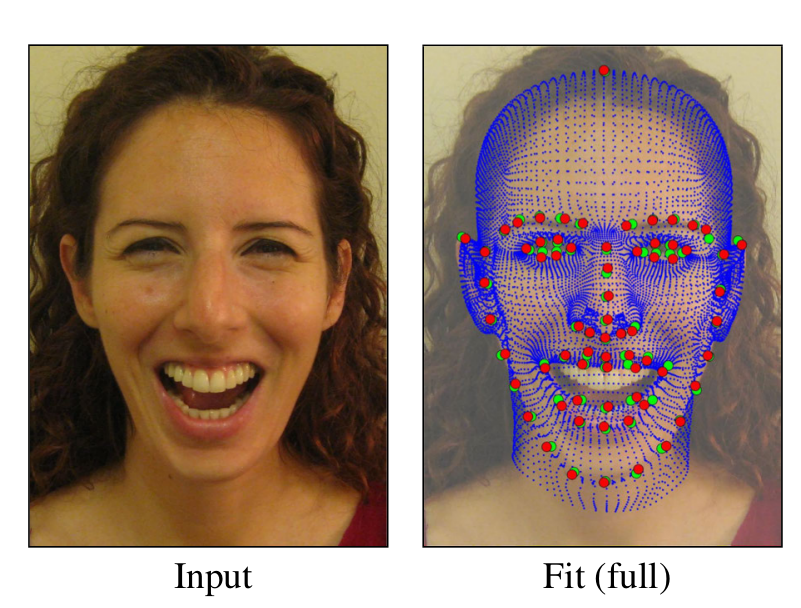
\includegraphics[width=0.5\textwidth]{img/perspective/fit.png}
	\end{figure}
}

\frame
{
	\frametitle{Perspective-aware Manipulation of Portrait Photos}
	
	\begin{figure}
		\centering
		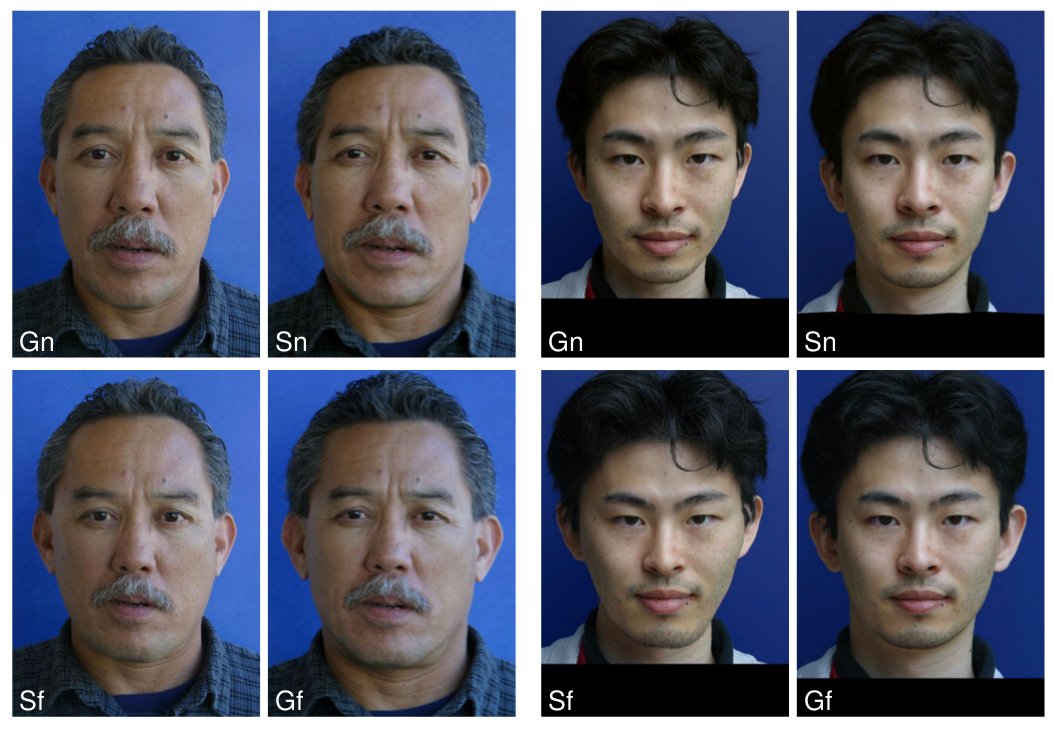
\includegraphics[width=0.9\textwidth]{img/perspective/results.png}
	\end{figure}
}

\frame
{
	\frametitle{Perspective-aware Manipulation of Portrait Photos}
	
	Applications:
	\begin{itemize}
		\item Distance correction
		\item Stereoscopy
		\item Pose correction
	\end{itemize}
}

\frame
{
	\frametitle{Perspective-aware Manipulation of Portrait Photos}
	
	\centering
	Demo\\
	\url{http://faces.cs.princeton.edu/demo/demo.html?input=0}
}